\subsubsubsubsection{Road sign name}
\begin{figure}[h]
\centering
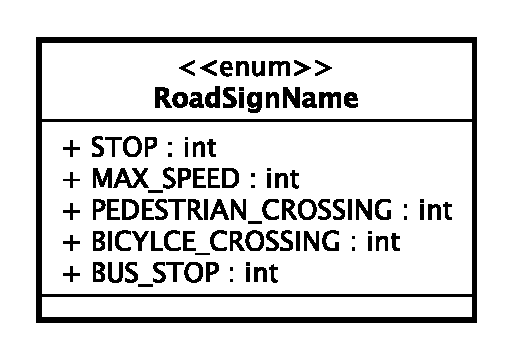
\includegraphics[scale=0.6,keepaspectratio]{images/solution/app/backend/road_sign_name.eps}
\caption{\pReactiveComponentStretchDecoration::RoadSignName}
\label{fig:sd-app-road-sign-name}
\end{figure}
\FloatBarrier
\begin{itemize}
  \item \textbf{\descr} \\
    It represents the name of a road sign.
  \item \textbf{\values}
  \begin{itemize}
    \item[+] \texttt{STOP: int} \\
	Notifies vehicles that they must stop before proceeding.
    \item[+] \texttt{SPEED\_LIMIT: int} \\
    Reveals the maximum speed at which road vehicles may legally travel.
    \item[+] \texttt{BUS\_STOP: int} \\
    Notifies a designated place where buses stop for passengers to board 
    or alight from a bus.
  \end{itemize}
\end{itemize}